\subsection{Models B.}
In this second case, given the symmetry of the problem, we have that, at equilibrium the deviatoric component of the stress tensor $\mathbb{T}$ vanishes. Combining this information with the boundary condition and solving the system~(\ref{sys1B})-(\ref{sys2B}) for its equilibrium, we obtain the same equations as for model A, while the pressure is now defined as:
\begin{equation}
p = \frac{\partial \psi_{vol}}{\partial J} .\label{presB}%= \frac{\kappa}{1+C_s v_s}.
\end{equation}

We follow two different approaches, in case $BA$, we derive the constitutive equation for $\psi_{vol}$, so that the model B and model A predict the same equilibrium behaviour, i.e. $p_A=p_{BA}$. Using Equations~(\ref{presA})-(\ref{presB}), and the constraint $\psi_{vol}(1)=0$, we obtain:
\begin{equation}
\frac{\partial \psi^{BA}_{vol}}{\partial J}= G^A_{eq} \frac{J^{2/3}-1}{J} \Longrightarrow \psi_{vol} = \frac{G_{vol}}{2}\left[3(J^{2/3} -1) - 2\ln J\right],
\end{equation}
which is equivalent to using a Neo-Hookean model also for the volumetric spring with shear modulus $G^{BA}_{vol}$. In the second case, we instead consider a more commonly used constitutive model for volumetric deformation. 

[ADD A FIGURE TO SHOW THE DIFFERENCE BETWEEN COLLAPSE AND HIGHLY SWOLLEN PHASE]
\section{Confined Compression Test.}

In this second example, we consider to perform on a swollen slice of ECM a compression test with the use of a porous platen,which allows the fluids to flow so to maintain the chemical equilibrium with the external bath \cite{Netti}. This allows to measure both the dynamical and equilibrium behaviour of the material by measuring the stress while imposing a known strain $\epsilon$. The corresponding deformation tensor is of the form:

\begin{figure}[h]
	\centering
	\def\svgwidth{0.89\linewidth}
	\input{latex/images/compression.pdf_tex}
	\vspace{2mm}
	\caption{Schematic representation of a compression test with a porous piston. A deformation is imposed in the $Z$ direction and the force necessary to maintain the deformation is recorded. }
\end{figure}
\begin{equation}
\F=J_0^{1/3}\begin{bmatrix}
1 &0&0\\
0&1&0\\
0&0& \lambda_1
\end{bmatrix},
\label{F} 
\end{equation}
where $\lambda_1 = 1 - \epsilon$. 
\subsection{Model A}
As before, given the symmetries of the system, $\B_e$ is a diagonal matrix of the form:
\begin{equation}
\B_e=\begin{bmatrix}
b &0&0\\
0&b&0\\
0&0& b_1
\end{bmatrix}. 
\end{equation}
Again we are here interested in the equilibrium behaviour, for which Equations~(\ref{eqion}) still holds. Focusing on the contribution of spring B, studying the equilibriums of Equation~(\ref{Be}), we obtain that $b=b_1$. Since $\det \B_e= (\det \F)^2$, we conclude that:
\begin{equation}
b = J_0^{2/3}\lambda_1^{2/3}.
\end{equation}

Using the boundary condition, we can now compute the pressure and the equilibrium condition:
\begin{gather}
p = -\sigma + \frac{G^A_1}{J_0\lambda_1} (J^{2/3}_0\lambda_1^2-1)+\frac{G^A_2}{J_0\lambda_1} (J_0^{2/3} \lambda_1^{2/3}-1) \\
\begin{aligned}
\frac{\sigma v_s}{k_B T}=&\frac{J_0\lambda_1+\chi}{J_0^2\lambda^2_1}+\frac{G_1^Av_s}{k_BT} \frac{J_0^{2/3}\lambda^2_1-1}{J_0 \lambda_1}+\frac{G_2^Av_s}{k_BT} \frac{J_0^{2/3}\lambda^{2/3}_1-1}{J_0 \lambda_1}\\[1.5mm]
&+\ln \frac{J_0\lambda_1-1}{J_0\lambda_1} +2c_0v_s-\sqrt{\left(\frac{z_fC_fv_s}{J_0\lambda_1-1}\right)^2+4v_s^2c^2_0}\label{compA}
\end{aligned}
\end{gather}

\subsection{Models B.}
Based on Equation~(\ref{F}), we have that the tensors $\bar{\B}$ and $\bar{\B}_e$ are of the form:
\begin{equation}
\bar{\B}=\begin{bmatrix}
\lambda_1^{-2/3} &0&0\\
0&\lambda_1^{-2/3}&0\\
0&0& \lambda_1^{4/3}
\end{bmatrix}, \qquad
\bar{\B}_e=\begin{bmatrix}
\bar{b} &0&0\\
0&\bar{b}&0\\
0&0& \bar{b}_1
\end{bmatrix}
\end{equation}

As for the model A, at equilibrium we have that $\bar{b}=\bar{b}_1$. However, in this case, we have that $\det \bar{B}_e=1$ so that $\bar{b}=1$ so that the second spring does not contribute to the stress. Using the boundary condition, in the case of model $BA$ we obtain:
\begin{gather}
\displaystyle 
p_{BA} = -\sigma + \frac{G_{vol}}{J_0\lambda_1}(J_0^{2/3}\lambda_1^{2/3}-1)+\dfrac{2G^B_1}{3J_0\lambda_1^{5/3}} (\lambda_1^2-1) \\
\begin{aligned}
\frac{\sigma v_s}{k_B T}=&\dfrac{J_0\lambda_1+\chi}{J_0^2\lambda^2_1}+\frac{2G_1^Bv_s}{3k_BT} \dfrac{\lambda^2_1-1}{J_0 \lambda_1^{5/3}}+\frac{G_{vol}v_s}{k_BT}\frac{J_0^{2/3}\lambda_1^{2/3}-1}{J_0\lambda_1}\\[1.5mm]
& +\ln \frac{J_0\lambda_1-1}{J_0\lambda_1}+2c_0v_s-\sqrt{\left(\frac{z_fC_fv_s}{J_0\lambda_1-1}\right)^2+4v_s^2c^2_0}.\label{compAB}
\end{aligned}
\end{gather}

Unlike the case of unconstrained swelling, we now have that the model $A$ and $BA$ are substantially different, so that there is no choice of the parameter that would predict the same stress-strain behaviour. This highlights how, the choice of a particular decomposition of the deformation gradient $\F$ correspond to a modelling decision on the constitutive properties of the material under study.  

\subsection{Model Comparison.}
\begin{figure}[h!]
	\begin{subfigure}{0.49\textwidth}
		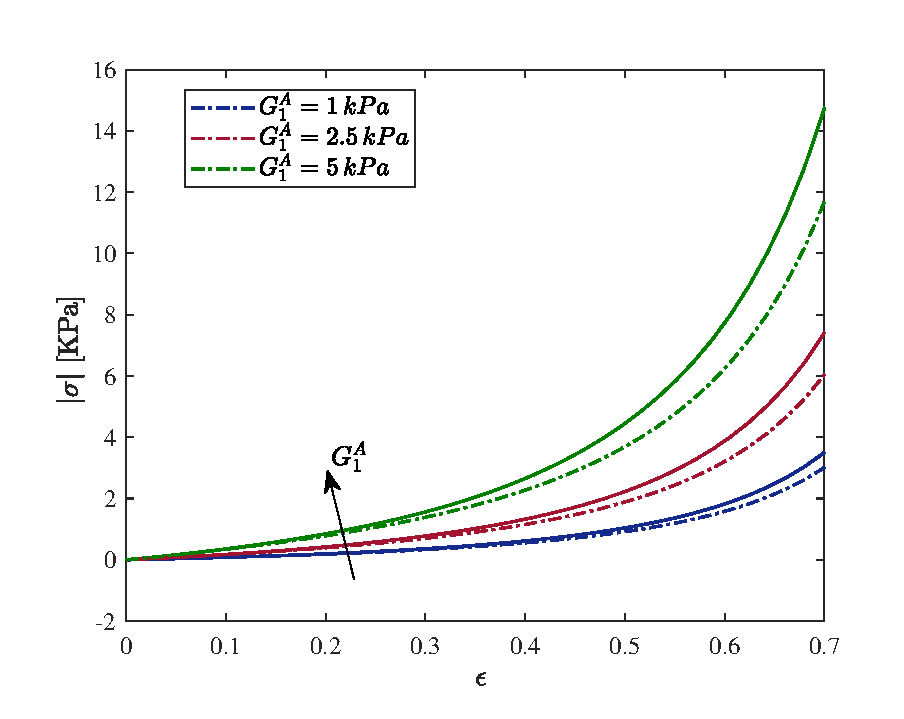
\includegraphics[scale=0.4]{images/comp1}
		\caption{}
	\end{subfigure}
	\begin{subfigure}{0.49\textwidth}
		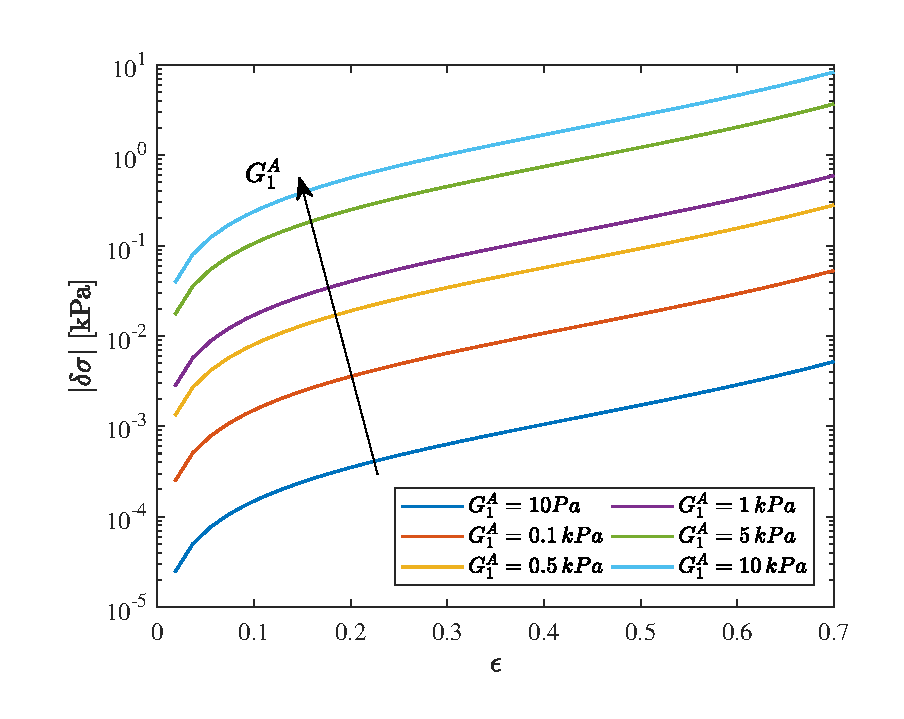
\includegraphics[scale=0.4]{images/comp2}
		\caption{}
	\end{subfigure}
	
	\begin{subfigure}{0.49\textwidth}
		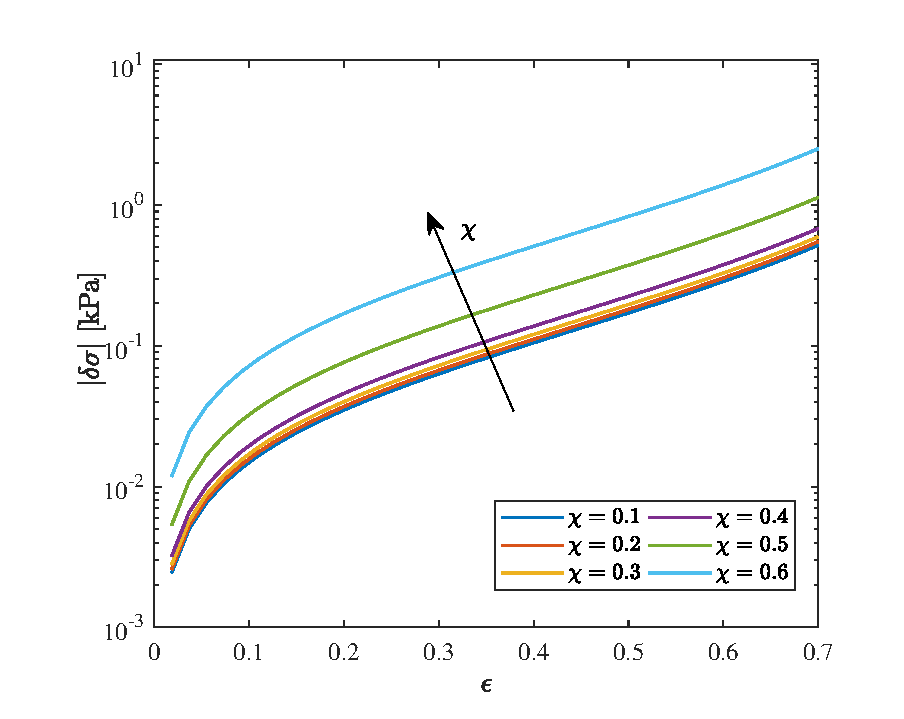
\includegraphics[scale=0.4]{images/comp3}
		\caption{}
	\end{subfigure}
	\begin{subfigure}{0.49\textwidth}
		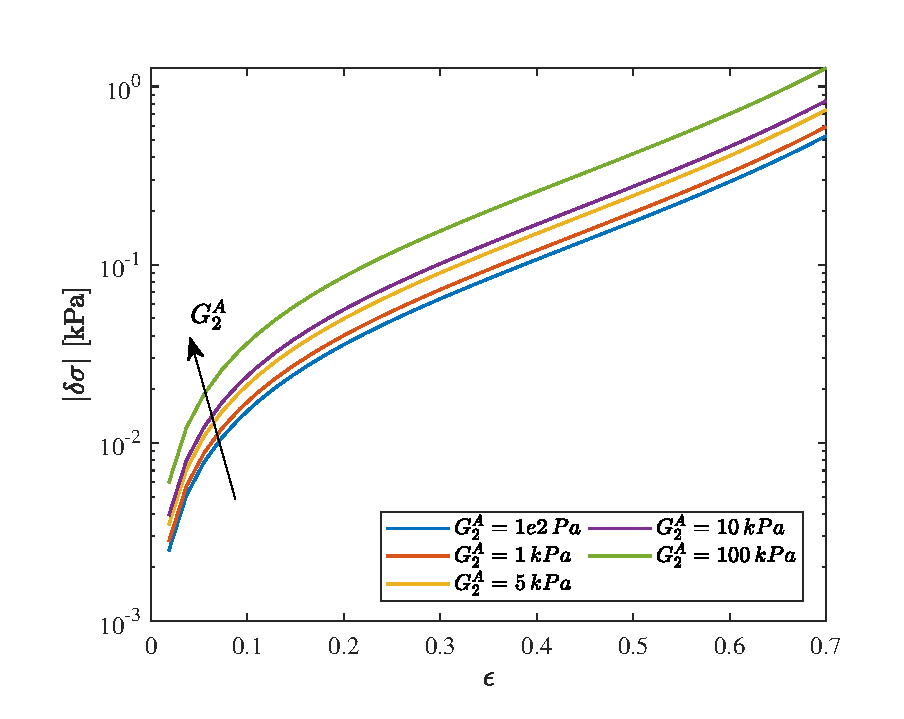
\includegraphics[scale=0.4]{images/comp4}
		\caption{CHANGE THE MAXIMUM OF THE PLOT}
	\end{subfigure}
	\caption{Sensitivity Analysis. As expected the mismatch between the two model grows with the strain: (a) Comparison of stress-strain curve predicted by model A (dotted line) and model B (full line) for different value of the parameter $G^A_1$; (b) as $G_1^A$ increase also the discrepancy $\delta\sigma$ grows; (c) $\delta\sigma$ is also particularly sensitive to changes in the mixing parameter $\chi$, in particular we see that there is a relevant jump when the ECM is the \textit{collapsed} phase; (d) on the other hand, only large changes in $G^A_2$ have a relevant impact on $\delta\sigma$.}
	\label{comp3}
\end{figure}
We first focus on comparing the model $A$ and $AB$, assuming that the parameter $\chi$ is fixed and that $G_{vol}=G^A_{eq}$, so that the equilibrium volume $J_0$ is the same for both models. If we now take the difference between Equations~(\ref{compA}) and (\ref{compAB}), we obtain that the difference in the compression stress $\delta \sigma= \sigma_{BA}-\sigma_{A}$ is:
\begin{equation}
\delta \sigma = \frac{2 G_1^{AB}}{3} \frac{\lambda_1^2-1}{J_0\lambda_1^{5/3}} - \frac{G_1^A}{J_0^{1/3}}(\lambda_1-\lambda_1^{-1/3}).\label{err}
\end{equation}
Looking at the above equation it appears clearly that there is no constant value of $G^{AB}_1$ for which the difference $\delta \sigma$ is identically zero. If we impose that for small deformation, i.e. $\lambda_1\rightarrow 1$, the two models agree at the second order:
\begin{equation}
\delta \sigma=0, \qquad \frac{\d \delta \sigma}{\d \lambda_1}=0 \quad\Rightarrow \quad G_1^{AB} = J_0^{2/3}G_1^A.
\end{equation}
Under such condition we can rewrite the Equation~(\ref{err}) as:
\begin{equation}
\delta \sigma(\lambda_1;G^A_1,J_0) = \frac{G_1^A}{J^{1/3}_0\lambda_1^{5/3}} \left(\frac{2}{3}\lambda^2_1-\frac{2}{3}-\lambda_1^{5/3}+\lambda_1^{4/3}\right), 
\end{equation}
which is unbounded for large deformation, i.e. $\lambda_1\Rightarrow0$. Note that $J_0$ is implicitly defined by Equation~(\ref{eqF}), where $J_0=1+v_sC_s$. Consequently $\delta\sigma$ depends also on all the other parameters of the problem. As shown in Figure \ref{comp3}, $\chi$ plays an important role in determining the agreement between the two models. In our analysis, we have deliberately decided to look at absolute instead of relative differences. This is because when study the mechanical properties of materials, the order of magnitude are relevant in particular for scaffolds where pressure regulates the response of cells.


%We here consider another standardd
\subsection{Test on Experimental Data.}
In the previous section we have compared the two models assuming that data on free swelling are also available, so that $G^A_{eq}$, or equivalently $G_{vol}$, can be estimated separately, with all the other parameter known. However, this is not usually the case. In particular, when testing real tissues already swollen $J_0$ is not known and needs also to be estimated. Moreover, at our knowledge there are no studies on the estimation of the mixing parameter $\chi$, so that this must be added to the list of unknown parameters. 

Using the data collected by Netti et~al. \cite{Netti}, we test the 
\begin{figure}[h]
	\hspace{-8mm}
	\begin{subfigure}{0.62\textwidth}
		\hspace{6mm}
		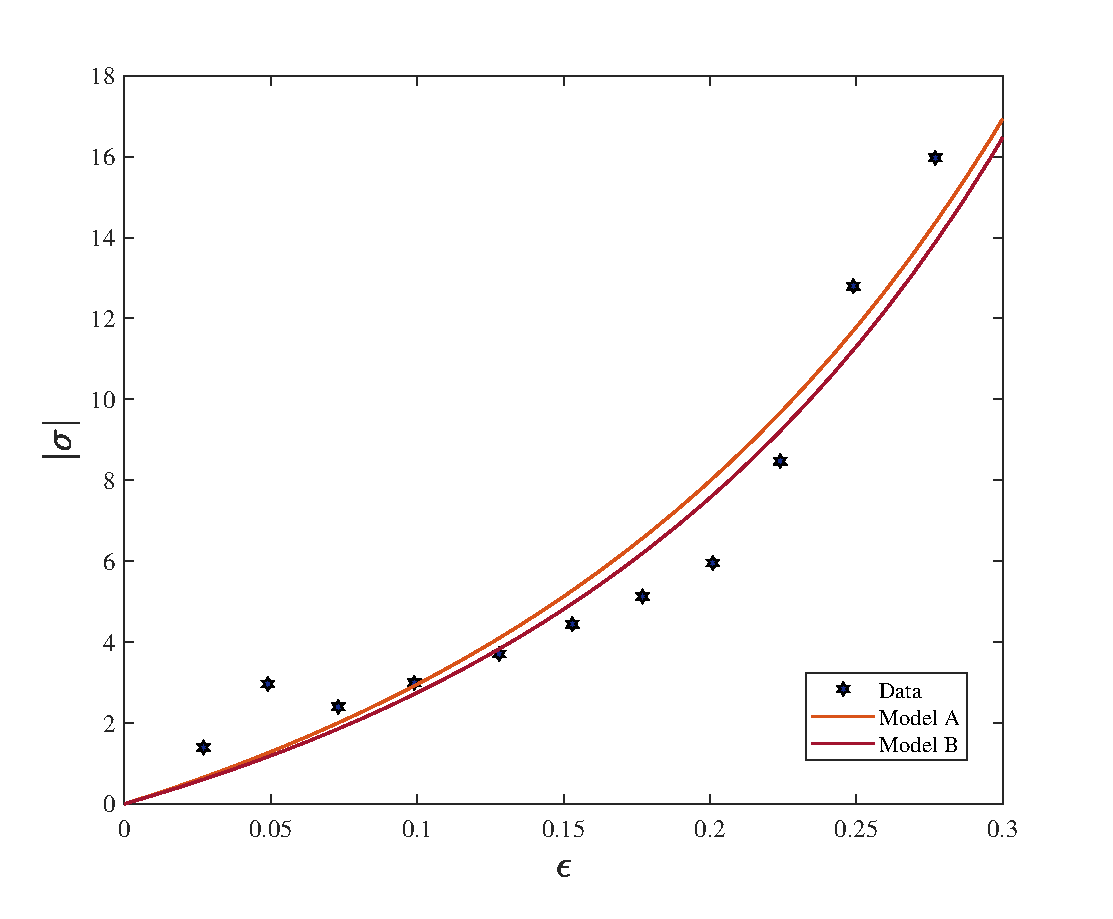
\includegraphics[scale=0.35]{images/compression.eps}
		\caption{Fitted Model}
		\label{fit}
	\end{subfigure}
	\begin{subtable}{0.375\textwidth}
			\begin{tabular}{c | c ||c| c }		
				\hline\addlinespace[2pt]
				 \multicolumn{2}{c||}{Model A} &  \multicolumn{2}{c}{Model AB}\\[0.5mm]
				\hline\addlinespace[2pt]
				$\quad \chi\quad$ & $\quad0.498\quad$ &$\quad \chi\quad$&$\quad0.524\quad$\\[0.5mm]
				$G^A_1$ & 18.9 kPa&$G_{vol}$&75 Pa\\[0.5mm]
				$G^A_2$ & 5.3 Pa&$G^{BA}_{1}$& 55.1 kPa\\[0.5mm]
				$J_0$ & $20.7$&  $J_0$&$14.8$\\[0.5mm]
				\hline
			\end{tabular}
		\caption{Estimated Parameters}
		\label{param}
	\end{subtable}
\caption{Comparison of the two model in fitting real experimental data from \cite{Netti}.}		
\end{figure}

As shown in Figure \ref{fit}, both models are able to capture the qualitative behaviour of the data. However, as shown by the parameters in Table \ref{param}, there are quantitative differences. In particular, there are order of magnitude of difference in the estimated pressure $p$. If we look at its value for zero-strain, i.e. $\lambda_1=1$, we obtain: 
\begin{gather}
p_A = \frac{G^A_1+G^A_2}{J_0}(J_0^{2/3}-1) = \frac{24.2 \text{ kPa}}{20.7}(20.7^{2/3}-1) = 7.64 \text{ kPa},\\
p_{BA} = \frac{G_{vol}}{J_0}(J_0^{2/3}-1) = \frac{0.075 \text{ kPa}}{14.8}(14.8^{2/3}-1) = 25.5 \text{ Pa}
\end{gather}

When designing synthetic ECM, the tuning of the internal pressure cells in a culture are exposed to is of large importance. As mentioned in the introduction, cells are sensitive to pressure and their response can greatly change depending on this stimulus. Consequently, depending on the model chosen, the
